\documentclass[crop,tikz, border=5pt]{standalone}
\usepackage{pgf}
\usepackage{tikz}
\usepackage{amsmath, amssymb}
\usetikzlibrary{arrows.meta}
\usetikzlibrary{arrows}
\usetikzlibrary{calc}
\usetikzlibrary{shapes}
\usepackage[utf8]{inputenc}


\begin{document}
    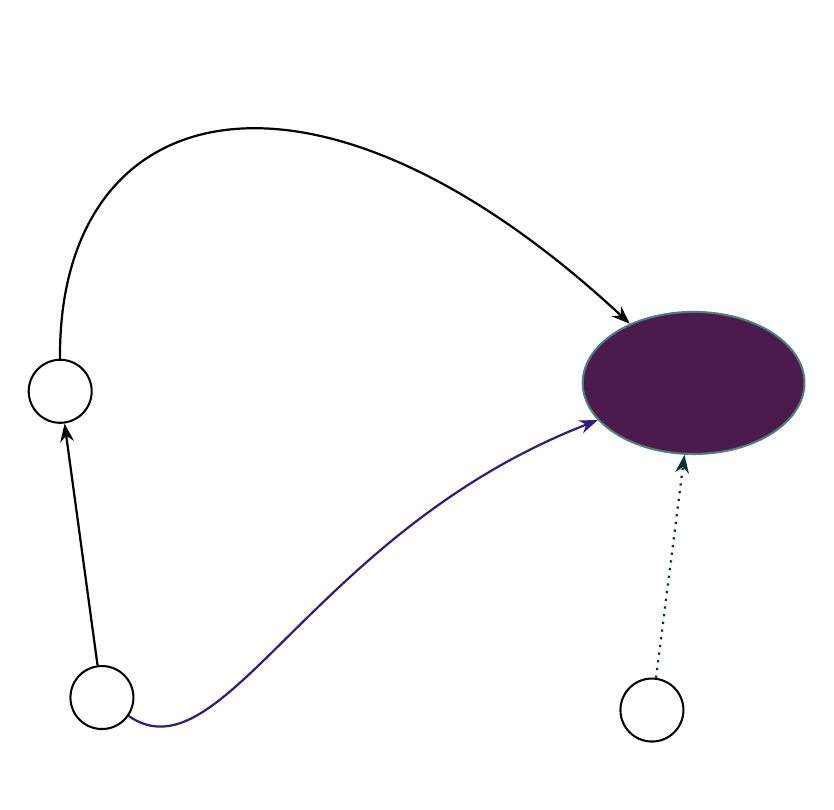
\begin{tikzpicture}[auto]
        \tikzset{>=Stealth}
        \tikzstyle{every path}=[->,thick]
        \tikzstyle{every node}=[ellipse,fill=white,draw=black,text=black,thin,minimum width=0.8cm,minimum height=0.8cm,inner sep=1.5pt]
        \tikzset{quadratic bezier/.style={ to path={(\tikztostart) .. controls($#1!1/3!(\tikztostart)$)
        and ($#1!1/3!(\tikztotarget)$).. (\tikztotarget)}}}

        \node [line width=0.026cm] (n0) at (4.503cm,-4.08cm) {};
        \definecolor{g-fillcolor}{HTML}{4D1A4D}
        \definecolor{g-strokecolor}{HTML}{4D8080}
        \node [minimum width = 2.816cm, minimum height = 1.805cm, fill=g-fillcolor, draw=g-strokecolor, line width=0.026cm] (n1) at (12.547,-3.974) {};
        \node [line width=0.026cm] (n2) at (12.018,-8.128) {};
        \node [line width=0.026cm] (n3) at (5.033,-7.969) {};

        \definecolor{g-fillcolor}{HTML}{003333}
        \draw [, g-fillcolor, dotted] (n2) to (n1);
        \draw [] (n3) to (n0);
        \draw [] (n0) .. controls (4.477,-0.296) and (7.705,--0.524) ..  (n1);
        \definecolor{g-fillcolor}{HTML}{331A80}
        \draw [, g-fillcolor] (n3) .. controls (6.567,-9.028) and (7.705,-5.853) ..  (n1);
    \end{tikzpicture}
\end{document}
